\documentclass{beamer}
\usetheme{Labsec}
\usepackage[utf8]{inputenc}
\usepackage[brazil]{babel}
\usepackage{graphicx}
\usepackage{listings}
\usepackage{wrapfig}
\usepackage{pgfpages}
\usepackage{ulem}

%\setbeameroption{show notes on second screen}
%\usepackage[width=3cm,tab]{beamerthemesidebar} % coloca a barra de navegacao lateral

\setbeamertemplate{navigation symbols}{} % tira a navegação}%C
\setbeamertemplate{footline}[frame number]

%%%%%%%%%%%%%%%%%%%%%%%%%
% Dados da Apresentação %
%%%%%%%%%%%%%%%%%%%%%%%%%
\title{An\'{a}lise e implementa\c{c}\~{a}o de um m\'{e}todo para prover integridade a sistemas de banco de dados}
\author{Gabriel Garcia Becker, Lucas Pandolfo Perin, Anderson Luiz Silv\'{e}rio, \\Marcelo Carlomagno Carlos, Ricardo Felipe Cust\'{o}dio}
\institute[LabSEC]{
  Laboratório de Segurança em Computação\\
  Universidade Federal de Santa Catarina\\[1ex]
  \texttt{\{gabrielbecker, lucasperin, anderson.luiz, custodio\}@inf.ufsc.br}
  \texttt{marcelo.carlos.2009@rhul.ac.uk}
  
}
\date{19 de Novembro de 2012}

% Mostra o sumario antes de cada nova secao
\AtBeginSection[]
{
\begin{frame}
\frametitle{\insertsection}
%\tableofcontents[currentsection,hideallsubsections]
%\tableofcontents[currentsection,hideallsubsections,subsection=hide]
\tableofcontents[sectionstyle=show/shaded,subsectionstyle=show/show/hide]
\end{frame}
}

%%%%%%%%%%%%%%%%%%%%
% INÍCIO DOCUMENTO %
%%%%%%%%%%%%%%%%%%%%
\begin{document}

%%%%%%%%%%%%%%%%%%%
% Slide de Titulo %
%%%%%%%%%%%%%%%%%%%
{
\usebackgroundtemplate{
\includegraphics[width=1.0\paperwidth]{images-template/watermark-logo.png}}
\begin{frame}[plain]
  \titlepage
\end{frame}
}
%%%%%%%%%%%%%%%%%%%%%%%%%%
% Slide de Sumario Geral %
%%%%%%%%%%%%%%%%%%%%%%%%%%
\frame{
	\frametitle{Sum\'{a}rio}
	\tableofcontents[hideallsubsections]
	%\tableofcontents
}

%%%%%%%%%%%%%%%%%%%%%%%%%%
%       Introducao       %
%%%%%%%%%%%%%%%%%%%%%%%%%%
\section{Introdução}
\frame{
  \frametitle{Motivação}
  \begin{itemize}
   \item \textit{Modificação não autorizada}
   \item Adição não autorizada
   \item Remoção não autorizada
   \item Consulta não autorizada
  \end{itemize}
  
  \begin{figure}[ht]
    	\begin{center}
		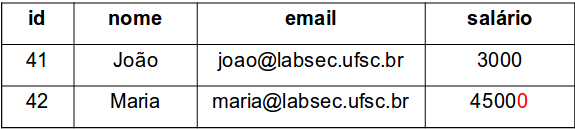
\includegraphics[width=0.6 \textwidth]{images/modificacao}
	\end{center}
  \end{figure}  
  
}

\frame{
  \frametitle{Motivação}
  \begin{itemize}
   \item Modificação não autorizada
   \item \textit{Adição não autorizada}
   \item Remoção não autorizada
   \item Consulta não autorizada
  \end{itemize}
  
  \begin{figure}[ht]
    	\begin{center}
		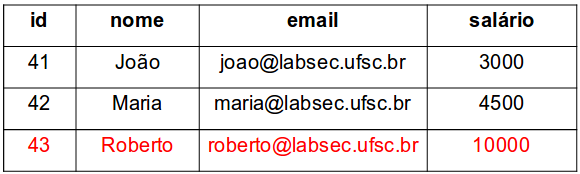
\includegraphics[width=0.6 \textwidth]{images/adicao}
	\end{center}
  \end{figure}  
  
}

\frame{
  \frametitle{Motivação}
  \begin{itemize}
   \item Modificação não autorizada
   \item Adição não autorizada
   \item \textit{Remoção não autorizada}
   \item Consulta não autorizada
  \end{itemize}
  
  \begin{figure}[ht]
    	\begin{center}
		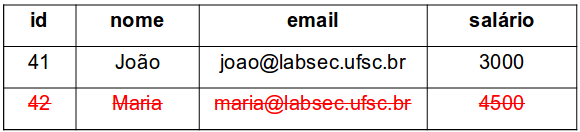
\includegraphics[width=0.6 \textwidth]{images/remocao}
	\end{center}
  \end{figure}  
  
}

\frame{
  \frametitle{Motivação}
  \begin{itemize}
   \item Modificação não autorizada
   \item Adição não autorizada
   \item Remoção não autorizada
   \item \textit{Consulta não autorizada}
  \end{itemize}
  
  \begin{figure}[ht]
    	\begin{center}
		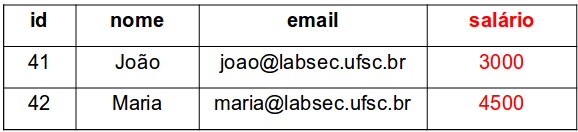
\includegraphics[width=0.6 \textwidth]{images/consulta}
	\end{center}
  \end{figure}  
  
}

\frame{
  \frametitle{Objetivos}
  \begin{itemize}
   \item Confidencialidade
   \item Integridade
   \item Autenticidade
   \item Rastreabilidade
  \end{itemize}
  
}




%%%%%%%%%%%%%%%%%%%%%%%%%%%%%%%%%
%  proposta  %
%%%%%%%%%%%%%%%%%%%%%%%%%%%%%%%%%
\section{Proposta}
\frame{
	\frametitle {Sigilo}
	\frametitle {Sigilo}
	\begin{figure}[ht]
	\begin{center}
	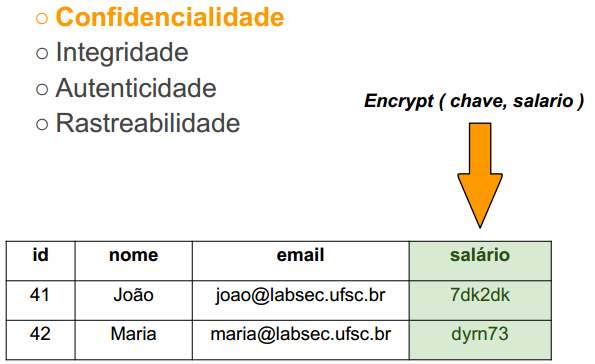
\includegraphics[width=\textwidth]{images/sigilo.png}
	\caption{Sigilo}
	\label{figura:sigilo}
	\end{center}
	\end{figure}
	
}

\frame{
	\frametitle {HMac}
	\begin{itemize}
	  \item Evitar a modificação não autorizada de registros contidos na base de dados.
	  \item Permite identificar as modificaçãos não autorizadas.
	\end{itemize}
		
}

\frame{
	\frametitle {HMac}
	
	\begin{figure}[ht]
	\begin{center}
	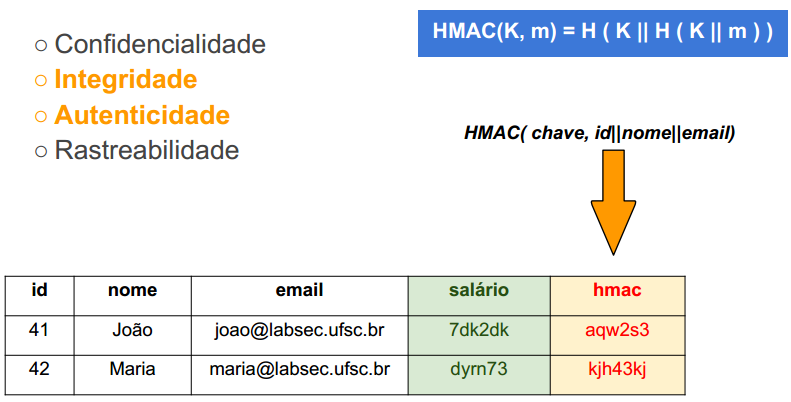
\includegraphics[width=\textwidth]{images/hmac.png}
	\caption{HMac}
	\label{figura:hmac}
	\end{center}
	\end{figure}
	
}

\frame{
	\frametitle {Histórico cifrado}
	\begin{itemize}
	  \item Com o HMac, não é possivel identificar remoções não autorizadas.
	  \item O Histórico Cifrado permite identificar as modificaçãos não autorizadas.
	  \item Permite relacionar dois ou mais registros de forma que possa se detectar a ausência de um deles.
	\end{itemize}

}

\frame{
	\frametitle {Histórico cifrado}
	\begin{itemize}
  	  \item Não permitir que uma terceira parte possa calcular o “histórico cifrado” sem conhecer as chaves de cifração.
  	  \item Utilização de operações de baixo custo computacional: criptografia simétrica e a operação lógica “ou exclusivo” (XOR);

	\end{itemize}

}

\frame{
	\frametitle {Histórico cifrado}
	
	\begin{figure}[ht]
	\begin{center}
	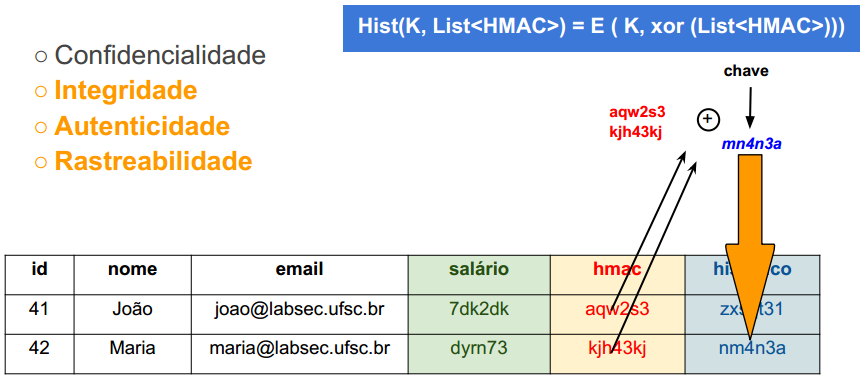
\includegraphics[width=\textwidth]{images/historico.png}
	\caption{Histórico Cifrado}
	\label{figura:historico}
	\end{center}
	\end{figure}

}


%%%%%%%%%%%%%%%%%%%%%%%%%%%%%%%%%
%  desempenho  %
%%%%%%%%%%%%%%%%%%%%%%%%%%%%%%%%%
\section{Desempenho}
\frame{
\frametitle {Desempenho}

\begin{table}[htb]\footnotesize
  \begin{center}
   \caption{Descri\c{c}\~{a}o do ambiente de simula\c{c}\~{a}o}.\label{tab:ambiente-simulacao}
    \begin{tabular}{l|l}
      \textbf{Processador} & Intel Core 2 Duo 2.53Mhz \\ \hline
      \textbf{Mem\'{o}ria RAM} & 4GB \\ \hline
      \textbf{Sistema Operacional} & Mac OS X 10.6.4 \\ \hline
      \textbf{Linguagem} & PHP 5.3 \\ \hline
      \textbf{SGDB} & MySQL 5.1 \\ \hline
      \textbf{Algoritmo de Hash} & SHA-1 \\ \hline
      \textbf{Tamanho de Chave HMAC} & 128 bits \\ \hline
      \textbf{Algoritmo de cifração} & AES 128 bits \\ \hline
      \textbf{Tamanho de chave sim\'{e}trica} & 128 bits \\
    \end{tabular}
  \end{center}
\end{table}

}

\frame{
\frametitle {Select, Insert, Updade e Delete}

\begin{figure}[ht]
\begin{center}
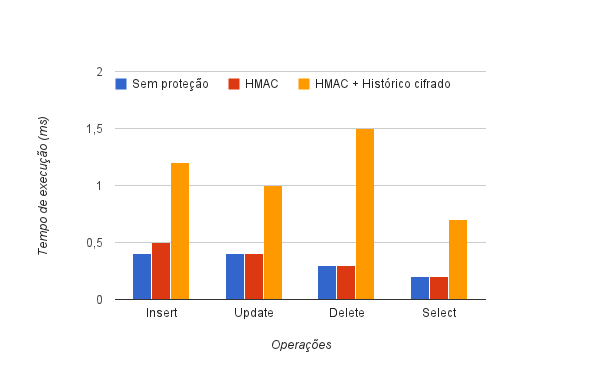
\includegraphics[width=\textwidth]{images/execucao1reg.png}
\caption{Tempo de execu\c{c}\~{a}o em segundos.} \label{figura:desempenho1reg}
\end{center}
\end{figure}

}

\frame{
\frametitle {Calculo em tabelas ja existentes}

\begin{figure}[ht]
\begin{center}
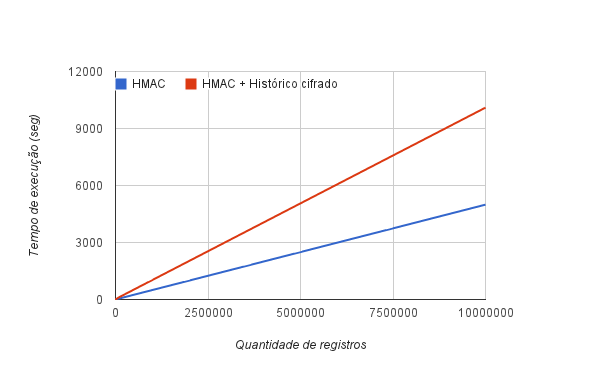
\includegraphics[width=\textwidth]{images/execucaoAdd.png}
\caption{Tempo de execu\c{c}\~{a}o em segundos.} \label{figura:desempenhoAdd}
\end{center}
\end{figure}

}

\frame{
\frametitle {Verificar integridade}

\begin{figure}[ht]
\begin{center}
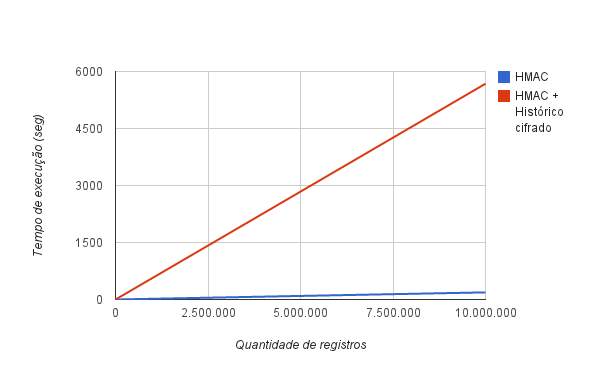
\includegraphics[width=\textwidth]{images/verificar.png}
\caption{Tempo de execu\c{c}\~{a}o em segundos.} \label{figura:verificar}
\end{center}
\end{figure}
}





%%%%%%%%%%%%%%%%%%%%%%%%%%
%     Implementação      %
%%%%%%%%%%%%%%%%%%%%%%%%%%
\section{Implementação}
\frame{
\frametitle {Biblioteca}

	\begin{figure}[ht]
	\begin{center}
	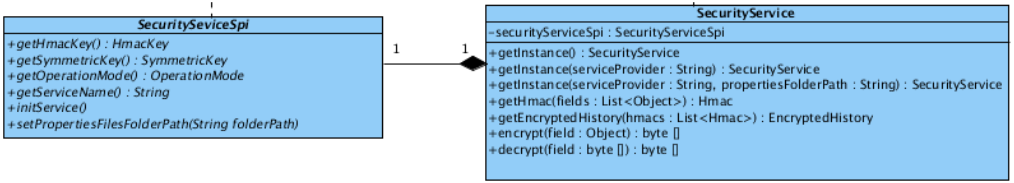
\includegraphics[width=\textwidth]{images/provider.png}
	\caption{Representa\c{c}\~{a}o do \textit{provider} da biblioteca} 			\label{figura:diagramProvider}
	\end{center}
	\end{figure}

}










%%%%%%%%%%%%%%%%%%%%%%%%%%
%       Conclusoes       %
%%%%%%%%%%%%%%%%%%%%%%%%%%
\section{Considerações finais}
\frame{
	\frametitle {Considerações finais}
	\begin{itemize}
          \item Desenvolvimento de método independente de SGBD.
          \item Testes mostram que o uso do HMAC é imperceptível na execução das operações básicas.
          \item Testes de operações em lote com tempos satisfatórios.
          \item Implementação de uma biblioteca.
	\end{itemize}
}

\frame{

\begin{center}
\LARGE
\item Perguntas?
\end{center}
}

\end{document}